
\documentclass[12pt]{article}
\usepackage{enumitem}
\usepackage{mathtools}
\usepackage{amsthm}
\usepackage{graphicx}
\graphicspath{ {images/} }
\begin{document}

\title{Assignment 2}
\author{Darwin Ding}
\maketitle

\section*{Exercise 1.8}
The probability of picking a marble out of the bag and getting red is 0.9, and we are looking for the probability that we sample 10 random marbles and get 1 or 0 red marbles.

The probability of getting 0 red marbles is $(.1)^{10} = 10^{-10}$, and the probability of getting 1 red marble is $(.1)^9 * .9 * 10$, because we pulled 9 green marbles (with probability .1) and 1 red marble (probability .9), and there were 10 ways to do that.

The probability of doing either of those things is the sum of those two probabilities is $\boldsymbol{9.1 * 10^{-9}}$

\section*{Exercise 1.9}
Using Hoeffding's Inequality, $\mu = .9$. Since we're looking for $v \le .1$, $\epsilon \ge .9 - .1 = .8$. By definition, also, $N = 10$.

\begin{gather*}
P[|v - \mu| \ge \epsilon] \le 2e^{-2\epsilon^{2}N}
\\ \le 2e^{-2 * .8^2 * 10}
\\ \le \boldsymbol{5.52 * 10^{-6}}
\end{gather*}

\section*{Exercise 1.10}
\begin{enumerate}[label=(\alph*)]
	\item After running the experiment a single time, $\mu$ for $v_0$ = \textbf{0.3}, $\mu$ for $v_{rand}$ = \textbf{0.5} and $\mu$ for $v_{min}$ = \textbf{0}
	\item 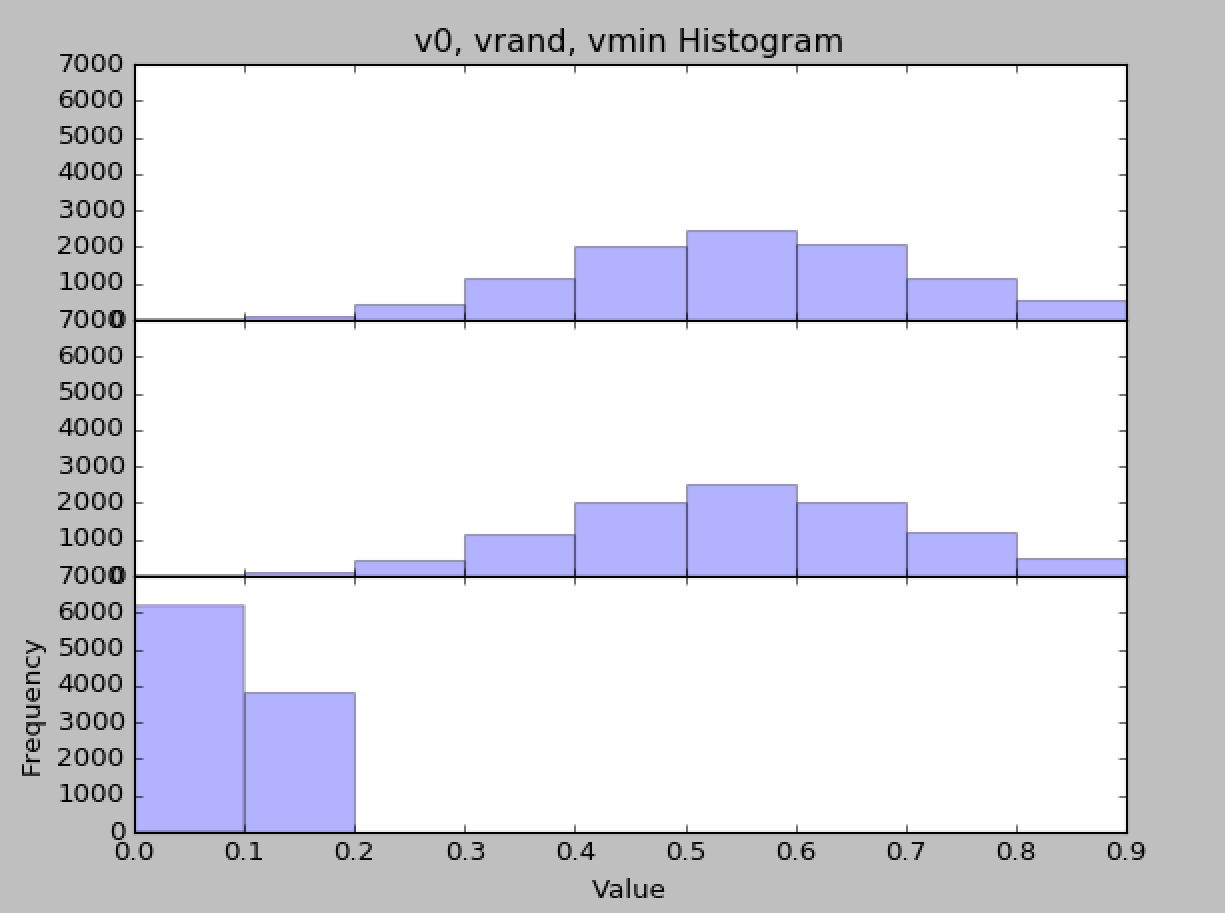
\includegraphics[scale=.5]{1-10-1.png}
	\\ The top graph is of $v_0$, the middle graph is $v_{rand}$, and the bottom one is $v_{min}$.
	\item 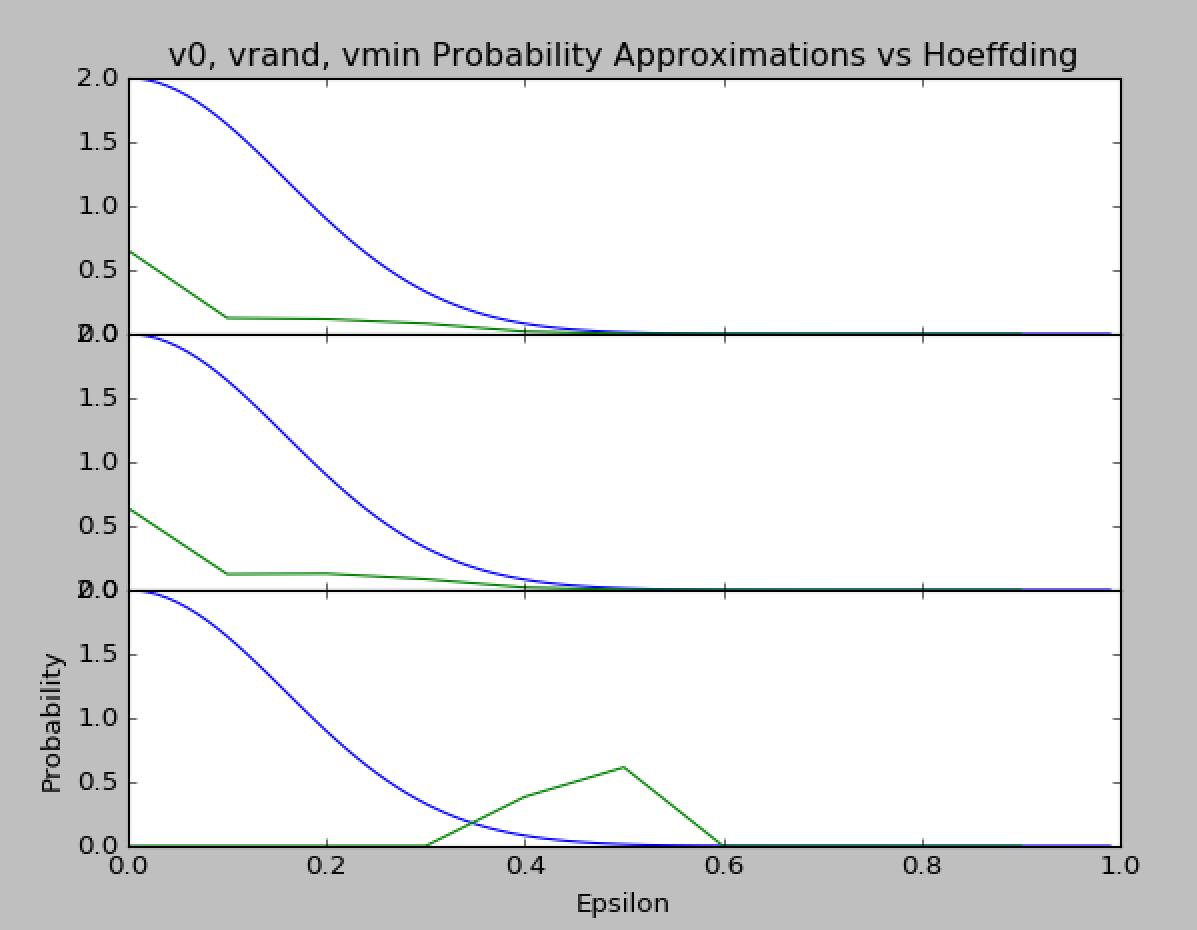
\includegraphics[scale=.5]{1-10-2.png}
	\\ Again, the top graph is of $v_0$, the middle graph is $v_{rand}$, and the bottom one is $v_{min}$. The green lines are the calculated estimates, and the blue lines are the plotted Hoeffding bounds.
	\item $v_0$ and $v_{rand}$ both obey the Hoeffding bound, while $v_{min}$ does not. This makes sense, because $v_0$ and $v_{rand}$ are essentially randomly selected coins. There's nothing special about the first coin or any random particular coin. The problem arises when you specifically seek out the minimum coin and then try to retroactively perform the Hoeffding bound. Hoeffding's inequality doesn't support this.
	\item If we pretend we don't know the true nature of coin flipping, and that $\mu$ is unknown to us, this problem is very similar to the bins problem. Let's say we are trying to predict $\mu$ using our data (the experiments we've performed and their results), and our hypothesis set is $[v_0, v_{rand}, v_{min}]$.
	\\ \\ If we fix our hypothesis set and then perform the experiment, we find that the Hoeffding bounds work simply because they work for $[v_0, v_{rand}]$. We cannot, however, claim that the bounds don't work simply because they retroactively don't work for $v_{min}$.
\end{enumerate}

\section*{Exercise 1.11}
\begin{enumerate}[label=(\alph*)]
	\item No, not necessarily. If $p = 0.5$, then even if $E_{in}$ is approximately equal to $E_{out}$, $E_{in} = 0.5$ which is just as good as random.
	\item Yes. Just because the smart algorithm has the smallest in-sample error (even if it's 0) doesn't mean there's a chance that the out-of-sample data is completely different from the in-sample. In this case, all of the points out of D might be -1, and the crazy learning algorithm will have worked better.
	\item If $p = 0.9$, S will pick the "correct" hypothesis unless $E_{in}(h_1) > 0.5$. The probability of that is the probability that $\epsilon > .4$ ($E_{out}(h_1) = .1$). M = 2, so this probability is bounded by $2 * 2 * e^{-2\epsilon^2N}$ = .0013. Therefore the probability that S correctly hypothesizes from the set is at least 1 - .0013 = \textbf{0.99866}
	\item For any p, $E_{in}(h_1) = 1 - p$. $E_{out}(h_1)$ needs to be on the opposite 'side' of $E_{in}$ with probability greater than 0.5 for the C algorithm to work. In other words, $|E_{out} - E_{in}| > \epsilon$, and $\epsilon = |p - 0.5|$.
	\\ \\ Solving for $2 * 2 * e^{-2(p - 0.5)^2*25} > 0.5$ gets us \textbf{0.296 $<$ p $<$ 0.704}
\end{enumerate}

\section*{Exercise 1.12}
The best you can provide is \textbf{(c)}. Depending on the problem, you may need to have a very large hypothesis set, which would decrease your out-of-bound prediction accuracy. In that scenario, you may have to announce that you have failed. However, if you find that $E_{out}$ is not close to 0.5, then you can announce that you have found a function that approximates well out-of-sample.

\section*{Problem 1.3}
\begin{enumerate}[label=(\alph*)]
	\item For separable data, the optimal set of weights will split the data such that for every point, $w^{*T}x_n$ has the same sign as $y_n$. If that is not true, then either the data is not separable or this is not the optimal set of weights. Since these all have the same sign, $\rho = w^{*T}x_n*y_n$ will always be positive for all n.
	\item According to the update rule, $w(t+1) = w(t) + y(t)x(t)$. Let's assume that we have some misclassified x(m) point with a corresponding y(m).
	\begin{gather*}
		w^T(t)w^* = w^{*T}(w(t-1) + x(m)y(m))
		\\ = w^{*T}w(t-1) + w^{*T}x(m)y(m)
	\end{gather*}
	$w^{*T}x(m)y(m)$ is positive for all n, so $w^{*T}x(m)y(m) \ge \rho$, since $\rho$ is the smallest in magnitude of all such n. Therefore, $w^T(t)w^* = w^{*T}w(t-1) + w^{*T}x(m)y(m) \ge w^{*T}w(t-1) + \rho$.
	\\ \\ \textbf{Base Case}
	\\ At t = 0, $w^T(t)$ is a vector of all 0s, and so both sides of the inequality are equal at 0.
	\\ \\ \textbf{Inductive Case}
	\\ At t = n, assume $w^T(n)w^* \ge t\rho$. At t = n+1, we've established in the previous portion that $w^T(n+1)w^* \ge w^{*T}w(t) + \rho \ge t\rho + \rho$.
	\\ \\ Therefore, $w^T(n+1)w^* \ge (t+1)\rho$ and the conclusion works.
	\item 
	\begin{gather*}
		||w(t)^2|| = ||(w(t-1) + x(t-1)y(t-1))^2||
		\\ = ||w(t-1)^2 + 2w^T(t-1)x(t-1)y(t-1) + x^2(t-1)y^2(t-1)||
		\\ = ||w(t-1)^2 + 2w^T(t-1)x(t-1)y(t-1) + x^2(t-1)||		
	\end{gather*}
	By definition, $||a|| + ||b|| \ge ||a + b||$. We know that $w^T(t-1)x(t-1)y(t-1) < 0$ simply because x(t-1) was selected because the PLA misclassified it at time t-1. Therefore:
	\begin{gather*}
		||w(t-1)^2 + 2w^T(t-1)x(t-1)y(t-1) + x^2(t-1)||
		\\ < ||w(t-1)^2 + x^2(t-1)||
		\\ \le ||w(t-1)||^2 + ||x(t-1)||^2
	\end{gather*}
	\item \textbf{Base Case}
	\\ At t = 0, $||w(t)||^2 = 0$, so both sides of the inequality are 0 again.
	\\ \\ \textbf{Inductive Case}
	\\ At t = n, assume $||w(t)||^2 \le tR^2$. At t = n+1, we've established in the previous portion that $||w(t+1)||^2 \le ||w(t)||^2 + ||x(t)||^2$. We also know that by definition, $x(t) \le R$ (meaning $||x(t)||^2 \le R^2$)
	\\ \\ Therefore, $||w(t+1)||^2 \le ||w(t)||^2 + ||x(t)||^2 \le tR^2 + R^2 = (t+1)R^2$ and the conclusion works.
	\item We know from (b), $w^T(t)w^* \ge t\rho$, and we know from (d), $||w(t)||^2 \le tR^2$, thus $||w(t)|| \le \sqrt{t}R$. This can be further transformed as follows:
	\begin{gather*}
		||w(t)|| \le \sqrt{t}R
		\\ 1/||w(t)|| \ge 1/(\sqrt{t}R)
	\end{gather*}
	Multiplying these two inequalities together, we find that $w^T(t)w^*/||w(t)|| \ge t\rho/(\sqrt{t}R) = \sqrt{t}\rho/R$. Squaring both sides, we get:
	\begin{gather*}
		w^T(t)w^*/||w(t)|| \ge t\rho/(\sqrt{t}R) = \sqrt{t}\rho/R
		\\ (w^T(t) * w^*)^2/||w(t)||^2 \ge t\rho^2/R^2
		\\ \frac{R^2(w^T(t) * w^*)^2}{\rho^2||w(t)||^2} \ge t
	\end{gather*}
	One key thing to note is that due to the definition of the dot product, where $A \cdot B = ||A|| ||B|| cos(\theta)$, $A \cdot B = A^T B \le ||A|| ||B||$ since $-1 \le cos(\theta) \le 1$. Therefore, we can further transform our equation as follows:
	\begin{gather*}
		\frac{R^2(||w(t)||*||w^*||)^2}{\rho^2||w(t)||^2} \ge \frac{R^2(w^T(t) * w^*)^2}{\rho^2||w(t)||^2} \ge t
		\\ \frac{R^2||w^*||^2}{\rho^2} \ge t
	\end{gather*}
\end{enumerate}

\section*{Problem 1.7}
\begin{enumerate}[label=(\alph*)]
	\item For 1 coin, the probability of getting no heads is equal to $\dbinom{10}{0}(1 - .05)^{10}$ = \textbf{0.598}
	\\ \\ For 1000 coins, we can use the previous result. P[at least 1 coin gets no heads] = 1 - P[all coins get at least 1 head] = $1 - (1 - .598)^{1000}$ which is approximately \textbf{1}
	\\ \\ We can continue this formula for 1,000,000, which will pretty much give us the same value: approximately \textbf{1}
	\item 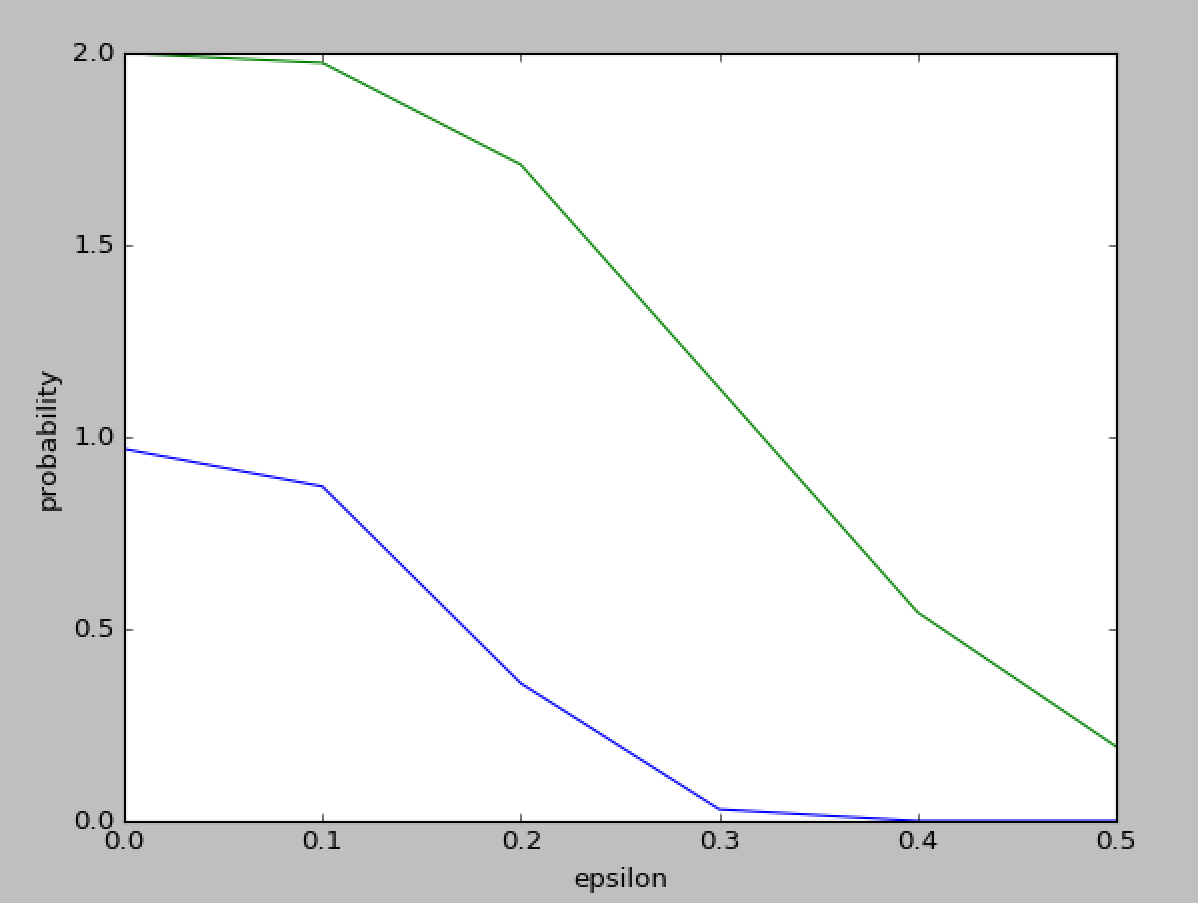
\includegraphics[scale=.5]{1-7-1.png}
	\\ The green line represents the Hoeffding bounds (calculated using P[coin 1 exceeds $\epsilon$] + P[coin 2 exceeds $\epsilon$] - P[coin 1 ...]P[coin 2 ...]), and the blue line represents the raw calculation from iterating and using the binomial expansion for each case.
\end{enumerate}
\end{document}